\documentclass[10pt, a4paper]{article}
%-----------------------
%- 	PACKAGES & SETTINGS
%-----------------------
\usepackage[utf8]{inputenc}
\usepackage[italian]{babel}
\usepackage{xcolor}
\usepackage{hyperref}
\hypersetup{
    colorlinks=true,
    filecolor=magenta,      
    urlcolor=darkgray,
    linkcolor=black
}
\urlstyle{same}
\usepackage{amsmath}
\usepackage{graphicx}
\graphicspath{ {images/} }
 
%-----------------------
%- 	TITLE
%-----------------------
\title{\textbf{Relazione Progetto Java PR 2}}
\author{\textbf{Venturi} Ludovico\\Docente: \href{http://pages.di.unipi.it/levi/}{Francesca Levi}}
\date{UNIPI, Novembre 2019}


%-----------------------
%- 	DOCUMENT
%-----------------------
\begin{document}
%- 	INTRO
\pagenumbering{roman} 
\maketitle
\tableofcontents
\vfill
\begin{figure}[h]
	\centering
	
\includegraphics[scale=0.07]{javaLogo}
	\label{fig:0}
\end{figure}

\clearpage

%- 	START DOC
\pagenumbering{arabic} 
\section{Scelte progettuali}
Nella relazione verranno spiegate le scelte progettuali e implementative che sono state prese.

\begin{figure}[h!]
	\centering
	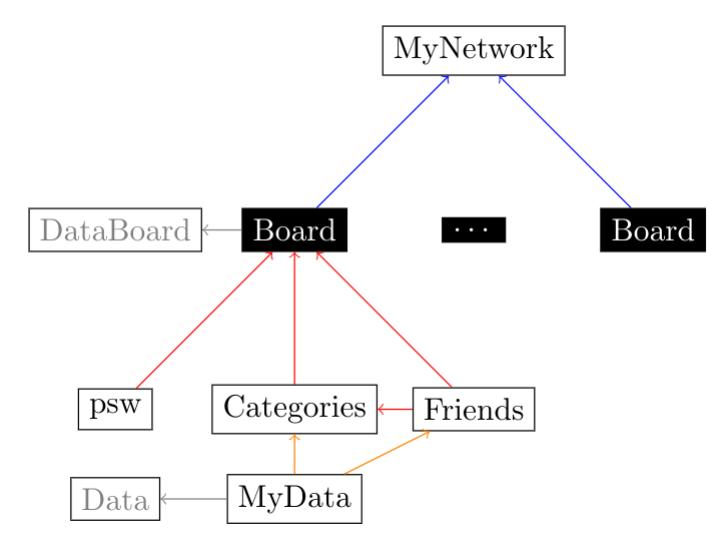
\includegraphics[scale=0.4]{diag1}
	\label{fig:diag1}
	\caption{Struttura generale del progetto comune ad entrambe le implemntazioni}
\end{figure}

\subsection{Data}
A grandi linee è stata creata una struttura generale dei dati in grado di adattarsi a varie situazioni.\\ \textit{Data} viene implementata come \textit{interfaccia}: stabilisce un \textit{contratto} con le sottoclassi che la implementeranno, ovvero: 
\begin{center}
OVERVIEW: \textit{Data rappresenta un dato astratto sottoforma di un insieme di 2 attributi e alcune operazioni. È una struttura astratta immutable, di dimensione finita e fissa}
\end{center}
Stabilisce delle caratteristiche comuni a tutte le sottoclassi: metodi che dovranno necessariamente implementare: 
\begin{center}
\textit{public void \textbf{display}();\\public String \textbf{getDataTitle}();\\public 		String \textbf{getCategory}();}
\end{center}
\subsubsection{MyData}
Viene poi implementata una sottoclasse \textit{astratta \textbf{MyData}} per soddisfare l'obiettivo iniziale di progettare una struttura versatile.\\
\textit{MyData} è implementata come classe astratta e tale scelta deriva dalla volontà di attribuire a tutte le classi che discendono da \textit{MyData} delle altre caratteristiche comuni, più \textit{concrete}, ovvero dei metodi già implementati e una struttura implementativa di base:
\begin{center}
	\textit{private String \textbf{dataName};\\
	private String \textbf{category};\\}
\end{center}
Come da specifica la classe \textit{MyData} riporta anche il metodo display , ma astratto: verrà implementato dalle sottoclassi.
Da \textit{MyData} discendono i dati veri e propri che saranno salvati in Bacheca: nell'esempio per il progetto sono \textit{Testo} e \textit{Audio}, che:
\begin{itemize}
	\item ridefiniscono \textit{equals()} per permettere la deep equality
	\item aggiungono un contenuto
	\item implementano display()
\end{itemize}

\subsubsection{Ipotesi}
\begin{itemize}
	\item La bacheca risulta una collezione di oggetti di vario tipo, come riportato nel testo, ma ciò non è collegato ad «E extends Data». Si è pertanto deciso di riportare anche la classe (magari apparentemente superflua) \textit{MyData} in modo da far trasparire chiaramente la presa di coscienza di ciò. La bacheca gestisce dati di tipo E : pertanto ogni dato sottotipo di E, con E definito come «E extends Data», è un dato valido da inserire in una bacheca basata sul tipo E.
	\item Non ci sono setter poichè si è ipotizzato che \textit{Data} fosse una struttura \textit{immutable}.
 \end{itemize}
 
\begin{footnotesize}
(Nel testo viene riportato «\textit{i dati possono essere
visualizzati dagli amici ma modificati solamente dal proprietario della bacheca}»: ciò è stato interpretato come: "la modifica consiste nell'aggiunta o la rimozione dei dati, non nella  modifica effettiva del contenuto dei dati").
\end{footnotesize}
\bigskip
\subsection{Board«E extends Data» }

\textit{Board} rappresenta un contenitore di oggetti generici. È basata sul tipo generico «E extends Data» e funzionalmente è una collezione di dati che possono essere di vario tipo, a patto che siano sottotipi di E (che estende \textit{Data}).

Non ho riportato la specifica di ogni metodo nel codice di \textit{Board(2)«E extends Data»} poichè risultava troppo confusionario; l'implementazione ha comunque seguito di pari passo la specifica riportata nell'interfaccia \textit{DataBoard«E extends Data»}.
\subsubsection{Ipotesi}
\begin{itemize}
\item Non sono ammessi elementi \textit{null}
\item Non sono ammessi duplicati di alcun genere
\item il numero di likes non dipende solamente dal dato ma anche dalla bacheca in cui si trova $\Rightarrow$ \textit{Data} non possiede il contatore dei like: questo si trova nella bacheca, relativamente ad ogni dato
\item la lista ritornata da \textit{getDataCategory} è in sola lettura, avendo precedentemente ipotizzato che Data sia immutable
\item la rimozione di una categoria comporta la perdita dei dati in quella categoria e l'associazione per ogni amico di quella categoria
\item i likes sono univoci per ogni amico
\paragraph{Nota sugli Iteratori} daie
\end{itemize}

\subsubsection{Implementazione 1}

\subsubsection{Implementazione 2}



\clearpage
\section{Eseguire il codice}
\subsection{Test ed esempi}
Non saranno verificate \textit{tutte} i casi in cui parametri sono null per ovvie ragioni, così come tutte le eccezioni ripetute, quali i controlli che la categoria esista o che l'amico sia presente nella lista amici; per queste ultime, pur se generabili in differenti metodi, verranno esplicitamente testate solamente una volta ciascuna. In generale più istruzioni su un singolo blocco \textit{try} indicano che l'ultima sarà quella che genera l'eccezione mentre le precedenti sono eseguite con successo.\\
Lista di test effettuati nel \textit{main}:
\begin{itemize}
\item password della bacheca « 8 caratteri
\item get di una bacheca non presente
\item password errata
\item stringa nulla passata (vale per tutti i metodi)
\item categoria già presente
\item rimozione di una categoria non presente
\item condivisione di una stessa categoria con uno stesso amico
\item condivisione di una categoria non presente nella bacheca
\item rimozione di un amico non presente nella lista amici
\item rimozione di un amico da una categoria cui non ha accesso, anche se presente nella lista amici
\item inserimento di un dato già presente
\item inserimento di un dato la cui categoria non è presente in bacheca
\item get di un dato la cui categoria non è presente
\item get di un dato non presente
\item get di un dato precedentemente inserito in modo corretto ma la cui categoria è stato poi rimossa
\item rimozione di un dato non presente
\item getDataCategory e modifica della lista ritornata
\item amico vuole inserire like ad un dato di una categoria non condivisa con lui
\item amico vuole inserire like ad un dato cui lo ha già messo
\item amico vuole inserire like ad un dato non presente
\item ITERATORI, prove varie
\item elimino una categoria e itero sui dati di tale categoria tramite una amico con cui essa era condivisa
\end{itemize}
% \href{www.multiplayer.it}{MULTIPLAYER}
% figura \ref{fig:im2} \pageref{fig:im2}
 
%\begin{itemize}
%  \item The individual entries are indicated %with a black dot, a so-called bullet.
%  \item The text in the entries may be of any %length.
%\end{itemize}

%$\begin{enumerate}



%\begin{equation}
%E=mc^2
%\end{equation}
%\subsection{daie}
%\label{sec:daie1}
%$ E=mc^2 $
%$\Omega + 3 = 54$\\
%$\omega * 54$

%\ref{table:tab1} SEZIONE \ref{sec:daie1}

%h = here
%\begin{table}[h]
%\centering
%\begin{tabular}{|c|c|r|}
%	\hline
%		cell1 & gatto & gattini \\
%	\hline
%		cell1 & gatto & 12 \\
%	\hline
%		cell1 & gatto & gattini \\
%	\hline
%\end{tabular}
%\label{table:tab1}
%\end{table}


\end{document}
